\section{Hybrid Programming} % using MPI+MPI$_{sm}$}

Most HPC systems in use today are clusters of shared memory nodes. The idea of hybrid programming consists of combining parallelization on the node interconnect with parallelization inside of each node. Traditionally, parallelization between nodes is being achieved using a distributed memory programming model such as MPI, while parallelization inside nodes is achieved using a shared memory programming model such as OpenMP, posix threads, or MPI$_{sm}$. 

\medskip
It has been recognized that getting good performance from a hybrid model can be difficult and requires understanding how the different programming models may interact \cite{UsingAdvancedMPI}. However, there are several reasons for using hybrid programing:

\begin{itemize} 

\item To reduce the memory footprint. Many codes require large lookup data structures that are global to the computation and ofter constant. For performance efficiency the data is ofter replicated at each process causing the memory demands of the application to grow with the number of processes. Sharing memory between MPI processes inside a node can often allow a way to share the data structure and keep only one copy per node instead of one copy per process. Nowadays this is becoming increasingly important since the number of cores in supercomputers is growing much faster than the number of nodes and than the amount of memory-per-core.

\item To improve performance. This could be achievable by directly accessing memory eliminating the need of communication through message passing between processes inside nodes.


\end{itemize}


\medskip

This section presents results of a parallel sparse matrix-vector multiplication (SPMV), a widely used operation in many simulations and the main kernel in iterative solvers, and compares its performance with and without using shared memory.


\medskip


\subsection*{Parallel SPMV}

The sparse matrix-vector multiplication (SPMV) consist in solving Equation \ref{eq:spmv}, where A is a sparse \emph{N X N} matrix and \emph{v} is a dense \emph{N}-dimensional vector \cite{BienzGO16}.


\begin{equation}
  w = A * v
\label{eq:spmv}  
\end{equation}

In parallel, the sparse system is often distributed across processes such that each process holds a contiguous block of rows from matrix \emph{A} and corresponding rows from vectors \emph{u} and \emph{w}. Within a single processes, it is common to splits the non-zeros values of the rows into two groups: an on-process block containing values associated to columns of the matrix that correspond to the part of vector \emph{v} values stored locally, and an off-process block containing the remainder of the non-zeros that are associated with vector \emph{v} values that are stored on other processes\cite{BienzGO16}. This is illustrated in Figure \ref{fig:Matrix}, for a case in which the matrix \emph{A} is divided among four processes. Different colors are used to illustrate the on-process block corresponding to each process. The same color is used to show the corresponding part of vectors \emph{w} and \emph{v}. In each process the off-process values of \emph{A} are on the remainder space, shown here without color.

\medskip

\begin{figure}[h!]
    \centering
    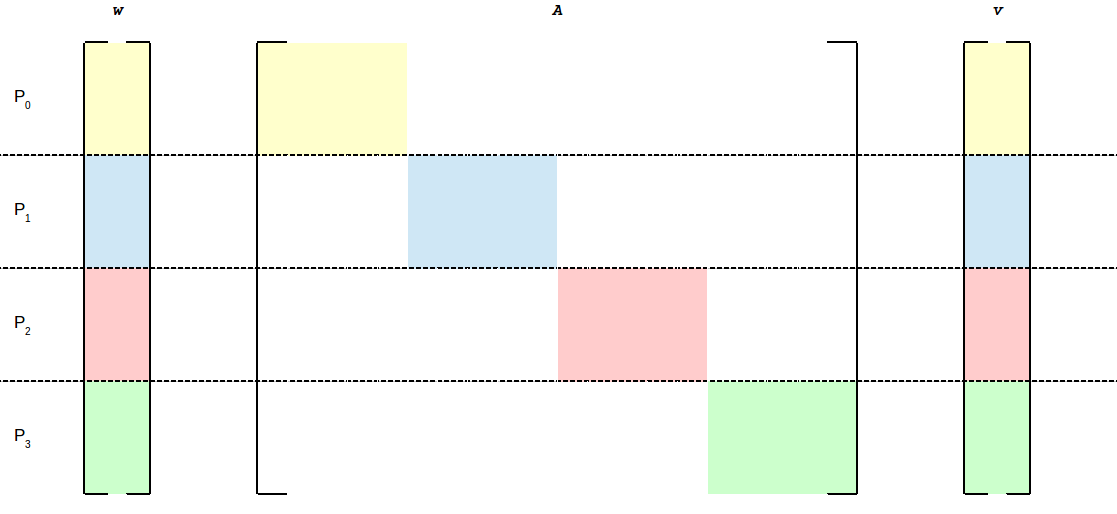
\includegraphics[width=100mm]{Plots/HybridProgramming/matrix.png}
    \caption{On-Proccess blocks shown in color.}
    \label{fig:Matrix}
\end{figure}

\medskip



With this configuration, the solution of equation \ref{eq:spmv} can be obtained by executing Equation (\ref{eq:spmv}) twice: once to solve using only the on-process block of matrix \emph{A} and the on-process part of the \emph{v} vector, and then, solve the equation again using the off-process block of matrix \emph{A} and elements of the \emph{v} vector held in other processes. These two partial solutions must be added to obtain the actual solution. While the first solution can be performed by each process independently, not requiring any communication among processes, the second solution require communication among the processes. For a more detailed explanation of this process the reader could take a look at \cite{BienzGO16}.

\medskip

It is known that, as the number of processes increases, the communication time start to dominate the execution time of the kernel. This is true even when communication is carefully overlapped with communication. As stated above, the communication part of this process consist in receiving parts of of the \emph{v} vector held in other processes. These parts have to be communicated using traditional send/receive calls even if both processes involved in the communication reside in the same node.

\medskip

Notice that the amount of communication of this kernel can be reduced if a process could have direct access to elements of the \emph{v} vector held in other processes. One extreme way to achieve this is by replicating the whole \emph{v} vector in each process; that would eliminate all the required communication. However, given that the \emph{v} vector is dense, this seems as an prohibitive alternative. Another possibility is if all the processes residing inside a node could have direct access to the parts of the \emph{v} vector already existing in the node. For example, referring to Figure \ref{fig:Matrix}, if the first two processes (yellow and blue) resides in a node while the last two processes (red and green) resides in a different node, 



The parallel spmv kernel seems as a good candidate to try a hybrid version of this algorithm. Returning to Figure \ref{fig:Matrix} 


